\chapter{Introduction}\label{chapter:introduction}

\nomenclature{Fig.}{Figure}
\nomenclature{$A_i$}{Area of the $i^{th}$ component}

% CONTENTS :
% 	Een situering van het onderwerp in een ruimere context. Dit kan, al naar gelang het onderwerp, vrij ver gaan: situering binnen het vakdomein, situering binnen de maatschappelijke evolutie, raakvlakken met andere disciplines,...
% 	Een beknopt historisch overzicht van de evolutie van het onderwerp.
% 	Een bespreking van bestaande oplossingen en systemen.
% 	De verklaring van de titel en dus ook definitie van de termen die gebruikt worden in de titel.
% 	De doelstellingen van de masterproef.
% 	Een overzicht van de verschillende hoofdstukken

Music catalogues for online retail have become immense over the past decades. In 2013 the iTunes music catalogue was comprised of over 26 million tracks with users downloading over 25 billion songs\cite{itunes:2013:sales}. Today virtually anyone can create music and upload it to a music database such as \emph{bandcamp}\footnote{\url{https://bandcamp.com/}}, \emph{iTunes}\footnote{\url{http://www.apple.com/itunes/}}, or \emph{Last.fm}\footnote{\url{http://www.last.fm/}}\cite{bandcamp:2013:artists, itunes:2013:sales, lastfm:2012:home}. Well-known artists and tracks make up a very small portion of this item space, which is known as the \emph{Long-tail phenomenon}\cite{levy:2010}. As a result, finding new, interesting music has become a challenging task. \emph{Recommender systems} try alleviate this problem by filtering the item repository based on a user's music taste. Taste can be modelled by analyzing user preferences and tracking user behaviour, e.g., by analyzing a user's listening history\cite{song:2012}.

Ever since computer engineers started to develop this kind of systems, a wide range of algorithms have been designed and implemented to compute item recommendations\cite{burke:2002, melville:2002:CCF:777092.777124, pazzani:2007:CRS:1768197.1768209, rajaraman:2012}; each of them with their own advantages and disadvantages.

There are two commonly applied recommendation strategies\cite{rajaraman:2012}:

\begin{itemize}
	\item \textbf{Content-based filtering (CBF)\nomenclature{CBF}{Content-based filtering}}: Using chosen or modelled features of items to define similarity between items in the user profile and candidate suggestions;
	\item \textbf{Collaborative filtering (CF)\nomenclature{CF}{Collaborative filtering}}: Using overlap of item sets of each user profile to find possible suggestions in the difference of these item sets.
\end{itemize}

Although recommender systems have proven to be successful in terms of prediction accuracy, the success of a recommender system also relies on the trust in its recommendations by the end user. If the user does not know why a particular item is recommended to him, the user may be reluctant to check it out. Herlocker et al. \cite{herlocker:2000} describe this issue as the \emph{black box problem}. To improve acceptance of recommendations, they propose to build an explanation system presenting the user with a \emph{white box model} of the recommender system rationale.

There are different ways in which explanation systems can be designed. An ambitious approach would be to explain each step of the recommendation algorithm, but this not always possible or desired. Other examples of how additional context can be provided for explainations are indicating which tracks in a user's music library are closely related to the given recommendations, giving the system's confidence in the accuracy of the suggestions, et cetera\cite{herlocker:2000}.

Over the course of the last decade a wide range of explanation systems have been implemented. Many of these also use visualizations to explore user and/or item relationships\cite{bostandjiev:2012, gou:2011:SIF:2016656.2016671, gretarsson:2010, odonovan:2008, zhao:2010}.


\section{Thesis objective}\label{chapter:introduction:section:objective}

The initial thesis objectives as described in \cite{kuleuven:2008:t313} are two-fold:

\begin{enumerate}
	\item The conduction of a literature study on techniques for the visualization of music suggestions;
	\item The design, implementation and evaluation of an interactive visualization that will allow the user to gain insight into the recommendation process as well as actively steer the process.
\end{enumerate}

The literature study describes recommender systems and their rationale, different visualization techniques, how users gain insight into visualization, and a number of visual explanation systems. In this context we will compose a new white box model that can be used as an explanation system for the collaborative recommendation rationale. This initial design is tested and improved through a number of iterations, resulting in an application that satisfies a number of criteria. These criteria are based on a set of evaluation properties, as described in the next subsections.

\subsection{Evaluation properties}\label{introduction:objective:properties}

The explanation system will be evaluated based on seven aims described by Tintarev and Masthoff \cite{tintarev:2007:SER:1547550.1547664} listed in table \ref{table:explanation:aims}. Also learnability (Learn.) and memorability (Mem.), properties of usability as described by Nielsen\cite{nielsen:1993:UE:529793}, are evaluated.

\begin{table}
	\caption{Explanation aims. Table adapted from Tintarev and Masthoff \cite{tintarev:2007:SER:1547550.1547664}.}
	\begin{tabular}{ p{130px} | p{300px} }
		\hline
		\textbf{Aim} 						& \textbf{Definition} \\
		\hline
		\textit{Transparency} (Tra.)		&	Explain how the system works. \\
		\textit{Scrutability}	(Scr.)		&	Allow users to tell the system is wrong. \\
		\textit{Trust}									&	Increase users' confidence in the system. \\
		\textit{Effectiveness} (Efk.)		&	Help users make good decisions. \\
		\textit{Persuasiveness}	(Pers.)	&	Convince users to try or buy. \\
		\textit{Efficiency}	(Efc.)			& Help users make decisions faster. \\
		\textit{Satisfaction} (Sat.)		& Increase the ease of usability or enjoyment. \\
		\hline
	\end{tabular}
	\label{table:explanation:aims}
\end{table}

\subsection{Evaluation methodology}\label{introduction:objective:methodology}

Transparency is tested by evaluating insight into the recommendation process based on North's evaluation method. We will use the think aloud protocol to obtain observational data. In particular we are looking for a user to make "domain specific inferences and hypotheses"\cite{north:2006}.

Satisfaction, efficiency, and learnability are tested through think aloud usability testing and a summative \emph{system usabiliy scale} (SUS) questionnaire. SUS is a \emph{Linkert scale} method consisting out of 10 questions, listed in figure \ref{table:sus_questions}, to investigate the subjective usability of an application\cite{brooke:1996}. Memorability is tested by asking test users that participated in previous iterations to explain the recommender rationale again at the beginning of the test.

\begin{table}
	\caption{System usability scale questions.}
	\begin{tabular}{ p{20px} | p{410px} }
		\hline
		\texttt{Q1} 	&	I think that I would like to use this system frequently. \\
		\texttt{Q2}		&	I found the system unnecessarily complex. \\
		\texttt{Q3}		&	I thought the system was easy to use. \\
		\texttt{Q4} 	&	I think that I would need the support of a technical person to be able to use this system. \\
		\texttt{Q5}		&	I found the various functions in this system were well integrated. \\
		\texttt{Q6}		&	I thought there was too much inconsistency in this system. \\
		\texttt{Q7} 	&	I would imagine that most people would learn to use this system very quickly.  \\
		\texttt{Q8}		&	I found the system very cumbersome to use. \\
		\texttt{Q9}		& I felt very confident using the system. \\
		\texttt{Q10}	& I needed to learn a lot of things before I could get going with this system. \\
		\hline
	\end{tabular}
	\label{table:sus_questions}
\end{table}

Trust, persuasiveness, and effectiveness are evaluated through direct feedback from the test subjects.

% The level of trust in the recommender system can provide an additional metric ---> not used in literature

\subsection{Success criteria}\label{introduction:objective:criteria}

We aim to build a system that is accessible to non-expert users. To achieve this, we hope to achieve positive results in terms of overal usability, learnability, memorability and transparency.

% + explain why these properties are relevant for non-expert users



\section{The visual explanation system}\label{chapter:introduction:section:application}

The application created for this thesis is a page action Chrome Extension that injects \emph{HTML} and \emph{JavaScript} into the recommendations page of \emph{Last.fm} at \url{http://last.fm/home/recs}. The application makes use of several \emph{JavaScript} libraries, such as D3\footnote{A library using SVG, HTML and JavaScript\cite{bostock:2012:d3js}; available at: \url{http://d3js.org/}} and jQuery\footnote{Available at: \url{http://jquery.com/}}, as well as a specific JavaScript library by Felix Bruns\footnote{Available at: \url{https://github.com/fxb/javascript-last.fm-api}} to facilitate the usage of the Last.fm API\footnote{Available at: \url{http://www.last.fm/api}}.

Figure \ref{figure:soundsuggest} shows the application. The application can be found in the Google Chrome web store\footnote{The SoundSuggest application can be found at: \url{https://chrome.google.com/webstore/detail/soundsuggest/jimmblcjmmjjfaklclmohcnabndlidmb}}.

\begin{figure}
	\begin{center}
		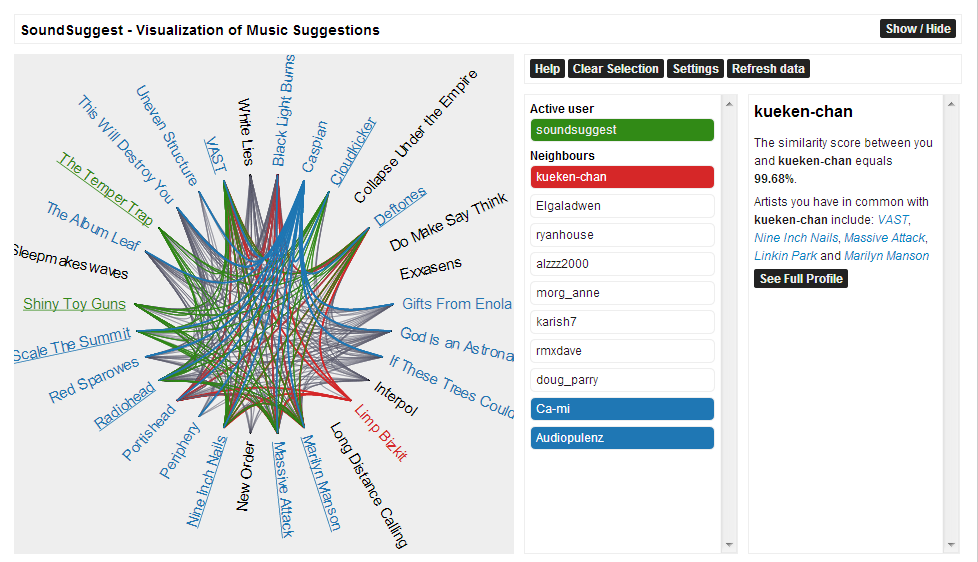
\includegraphics[width=\columnwidth]{img/soundsuggest}%
	\end{center}
	\caption{The \emph{SoundSuggest} application.}
	\label{figure:soundsuggest}
\end{figure}


\section{Next chapters}\label{chapter:introduction:section:chapters}

The rest of this thesis text is organized as follows. Chapter \ref{chapter:literature_study} presents a literature study on recommender systems, visualization techniques, insight gaining and visual explanation systems. Chapter \ref{chapter:requirements} tries to identify the target audience and how the application can be used. Chapter \ref{chapter:prototype} describes the testing methodology and the different iterations. Chapter \ref{chapter:implementation} looks at the technologies that were used to develop the application and the architecture of the application, and discusses some of the specifics of the implementation. Chapter \ref{chapter:conclusion} concludes the thesis text. It provides an interpretation of the application's evaluation results, further conclusions, and a reflection on future work and opportunities.
